\begin{figure}[!h]
	\begin{center}
    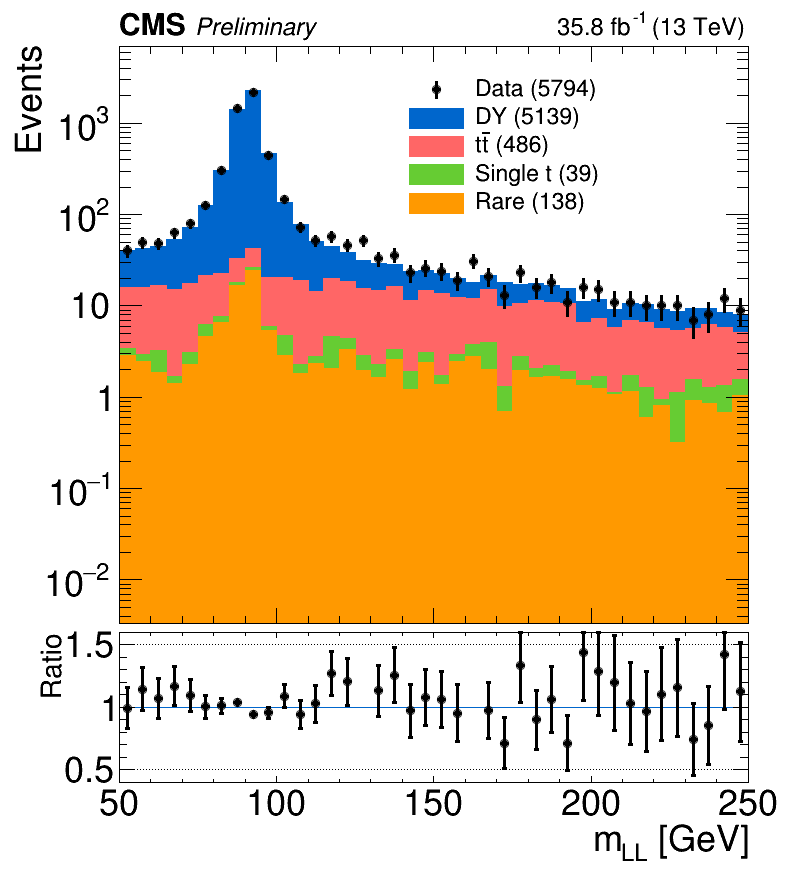
\includegraphics[width=0.40\textwidth]{znunu/fromCaleb/DataMC_Muon_LowDM_bestRecoZM_50to250_jetpt30_2016.png} \\
    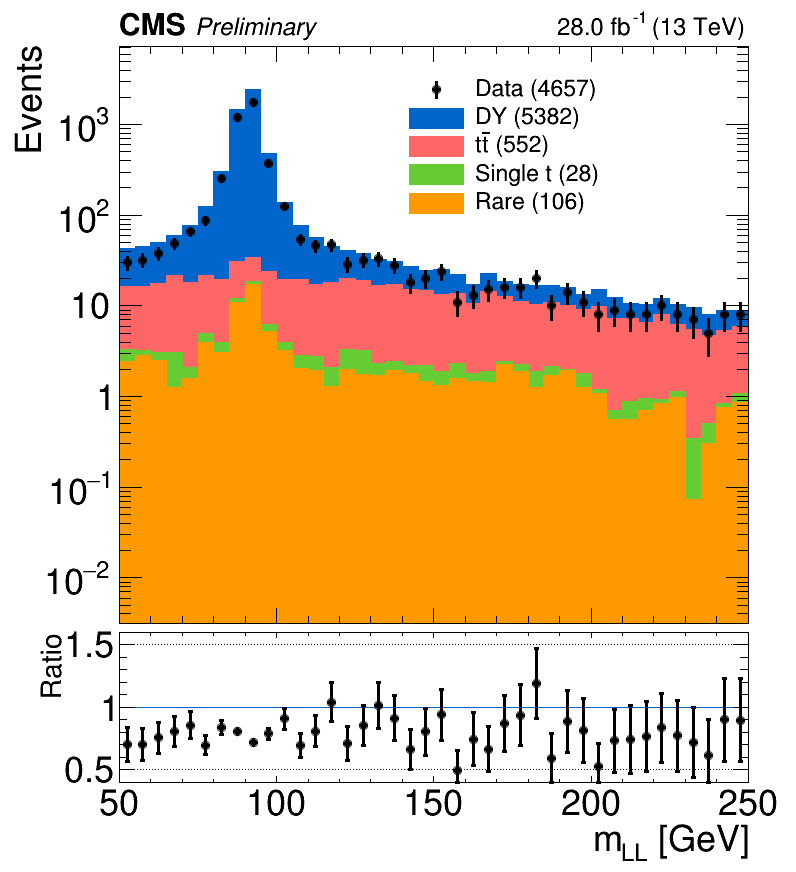
\includegraphics[width=0.40\textwidth]{znunu/fromCaleb/DataMC_Muon_LowDM_bestRecoZM_50to250_jetpt30_2017_BE.png} 
    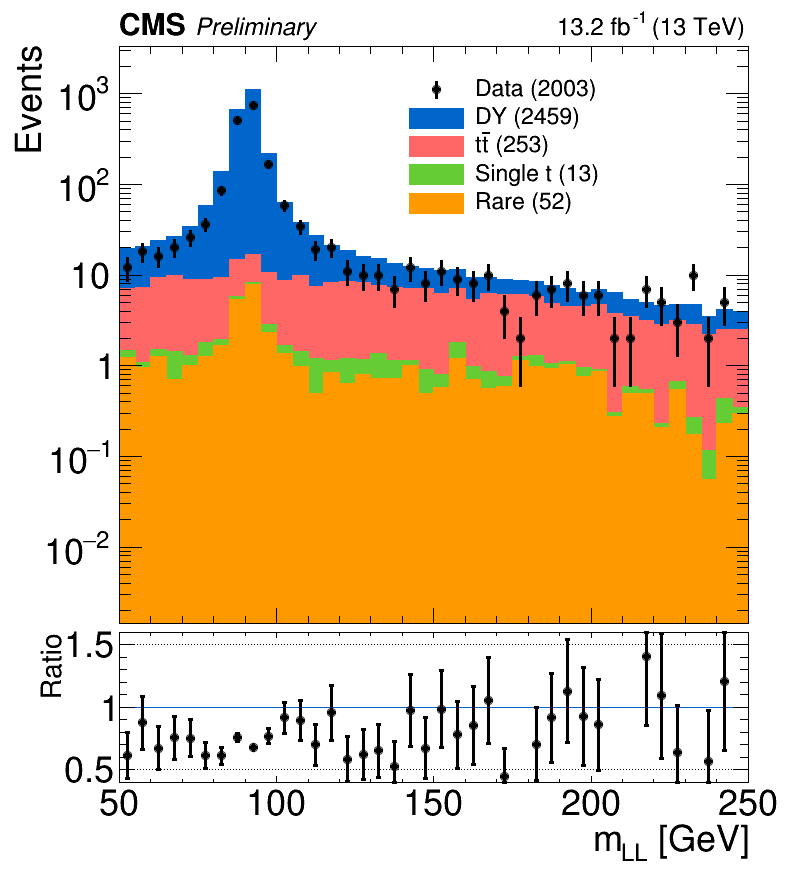
\includegraphics[width=0.40\textwidth]{znunu/fromCaleb/DataMC_Muon_LowDM_bestRecoZM_50to250_jetpt30_2017_F.png} \\
    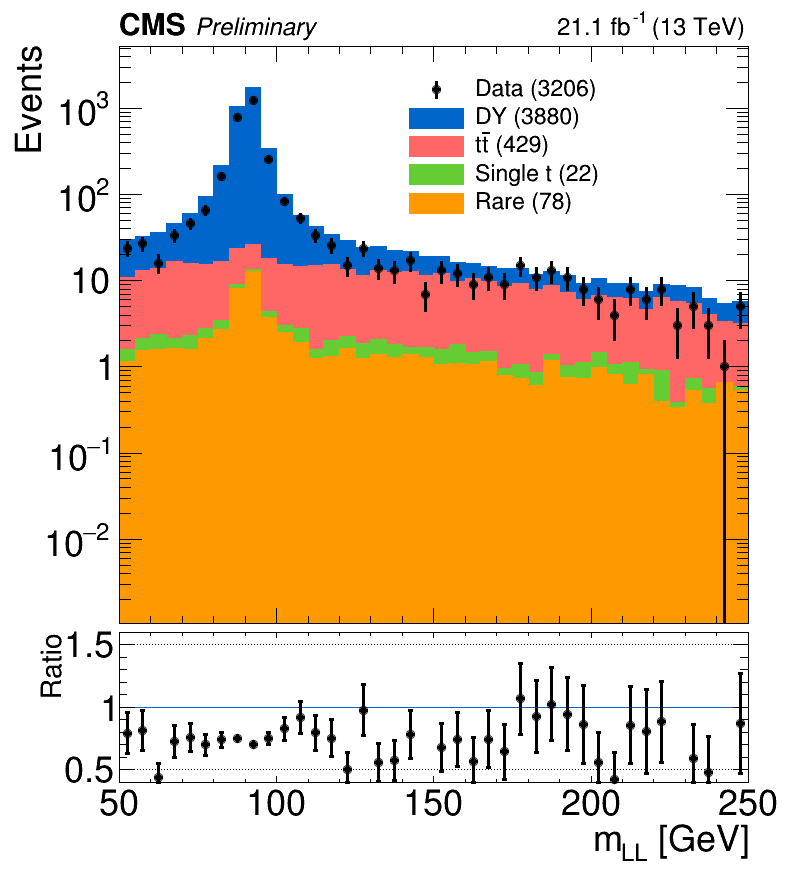
\includegraphics[width=0.40\textwidth]{znunu/fromCaleb/DataMC_Muon_LowDM_bestRecoZM_50to250_jetpt30_2018_PreHEM.png}
    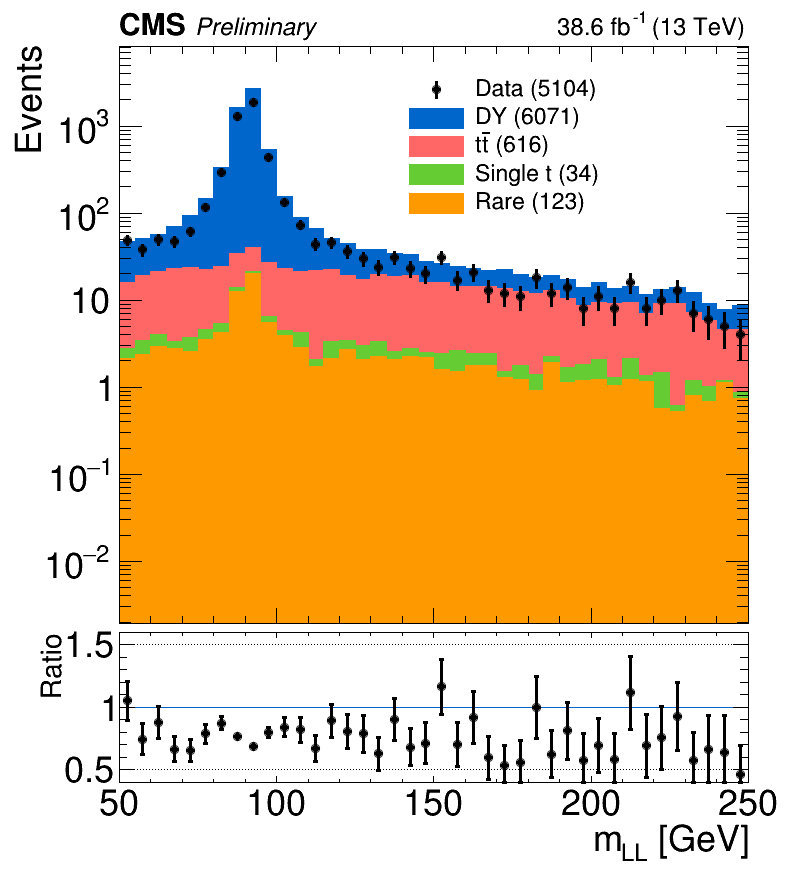
\includegraphics[width=0.40\textwidth]{znunu/fromCaleb/DataMC_Muon_LowDM_bestRecoZM_50to250_jetpt30_2018_PostHEM.png} \\
	\end{center}
	\caption[\Znunu{} Normalization in Low \dm{} for Muons]{The \Znunu{} normalization separated by era for the muon control region. The selection is the low $\dm, \nb=0, \nsv=0$ in the muon control region.
	 }
	\label{fig:znunu-norm-lm-muon}
\end{figure}

\begin{figure}[!h]
	\begin{center}
    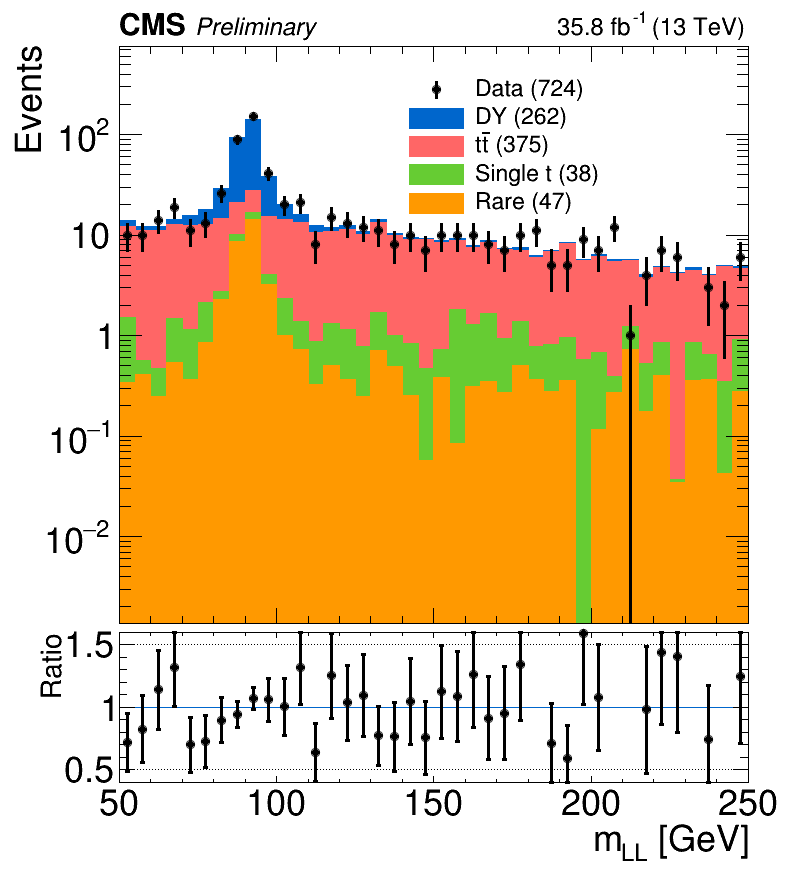
\includegraphics[width=0.40\textwidth]{znunu/fromCaleb/DataMC_Muon_HighDM_bestRecoZM_50to250_jetpt30_2016.png} \\
    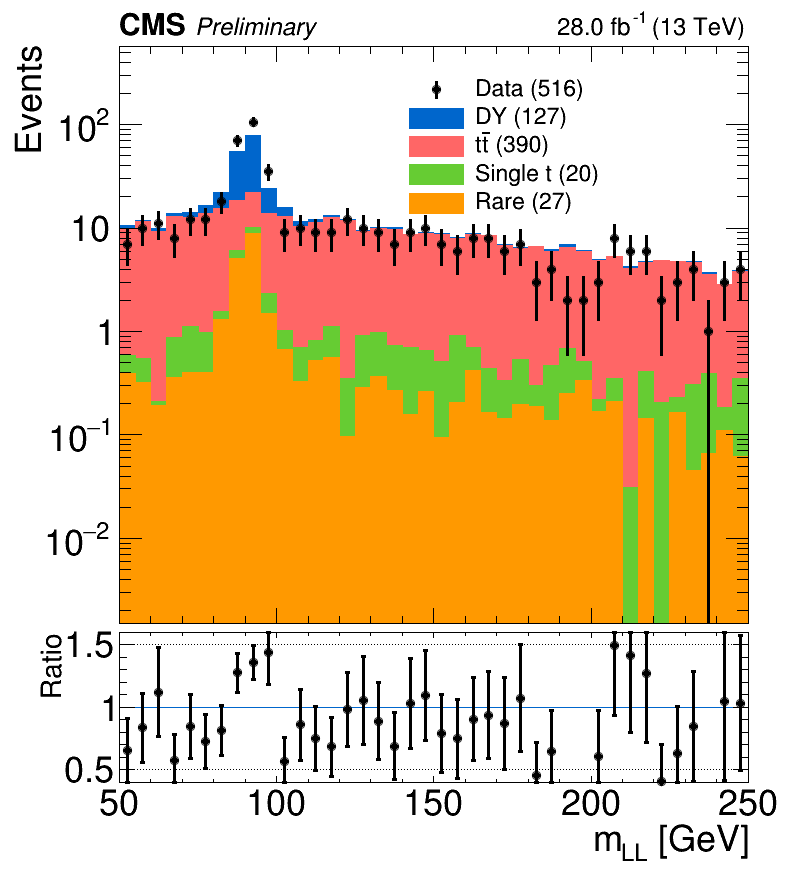
\includegraphics[width=0.40\textwidth]{znunu/fromCaleb/DataMC_Muon_HighDM_bestRecoZM_50to250_jetpt30_2017_BE.png} 
    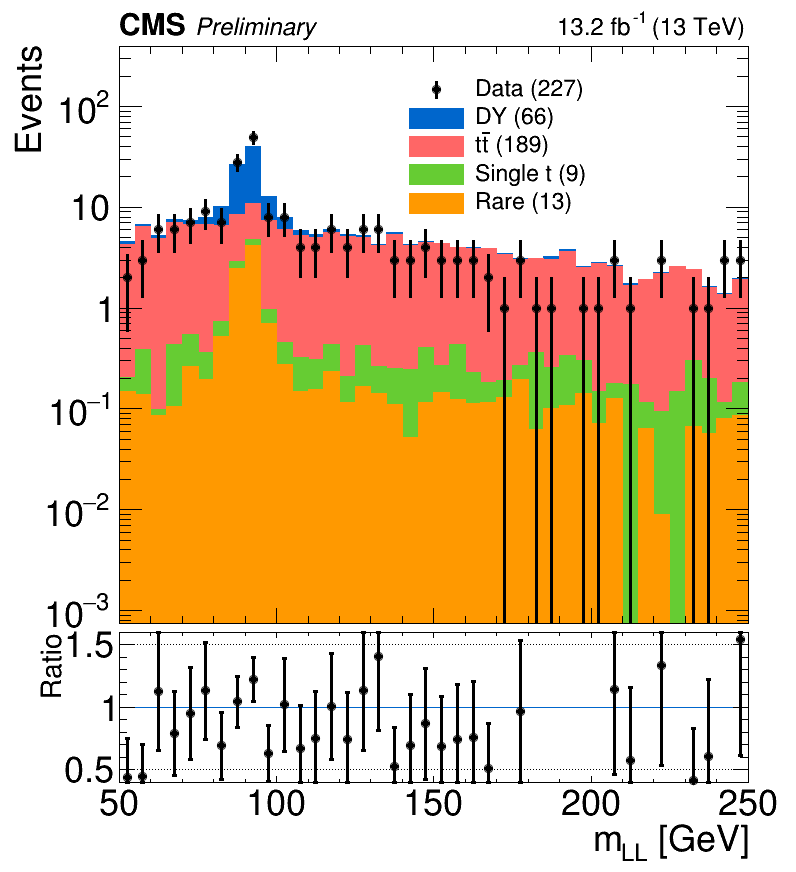
\includegraphics[width=0.40\textwidth]{znunu/fromCaleb/DataMC_Muon_HighDM_bestRecoZM_50to250_jetpt30_2017_F.png} \\
    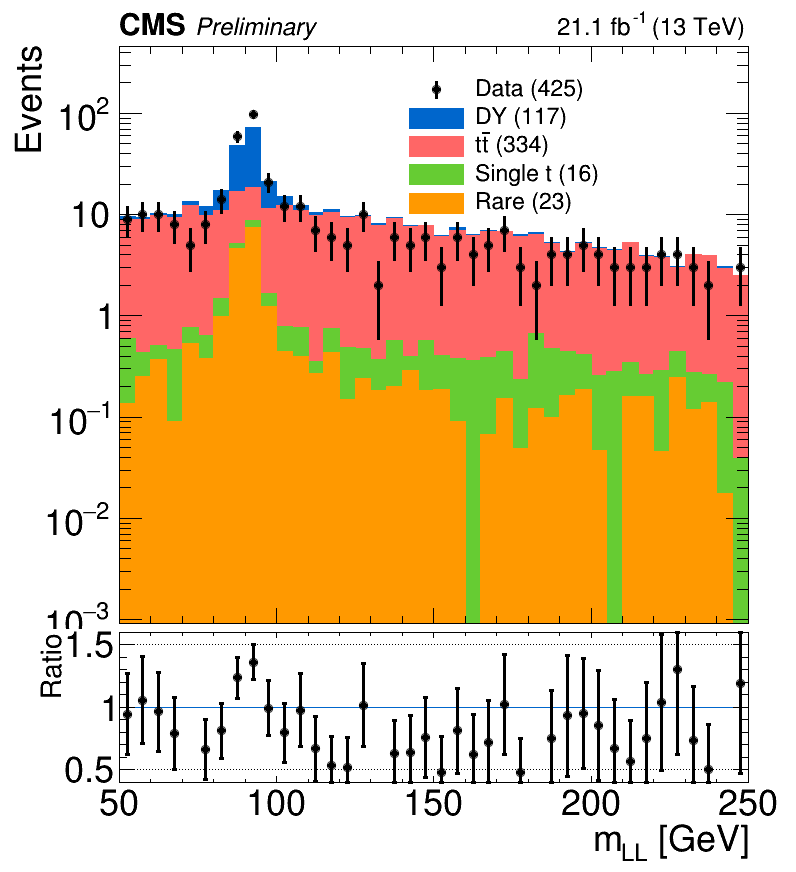
\includegraphics[width=0.40\textwidth]{znunu/fromCaleb/DataMC_Muon_HighDM_bestRecoZM_50to250_jetpt30_2018_PreHEM.png}
    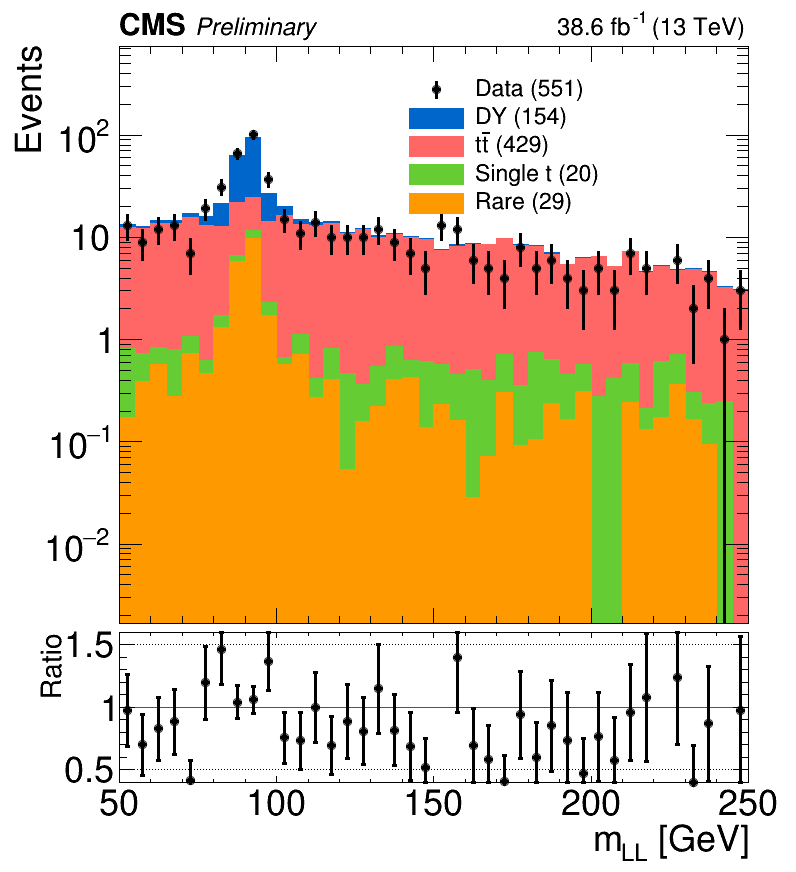
\includegraphics[width=0.40\textwidth]{znunu/fromCaleb/DataMC_Muon_HighDM_bestRecoZM_50to250_jetpt30_2018_PostHEM.png} \\
	\end{center}
	\caption[\Znunu{} Normalization in High \dm{} for Muons]{The \Znunu{} normalization separated by era for the muon control region. The selection is the high $\dm, \nb=1, =2, \geq2,\geq3$ in the muon control region.
	 }
	\label{fig:znunu-norm-hm-muon}
\end{figure}

\begin{figure}[!h]
	\begin{center}
    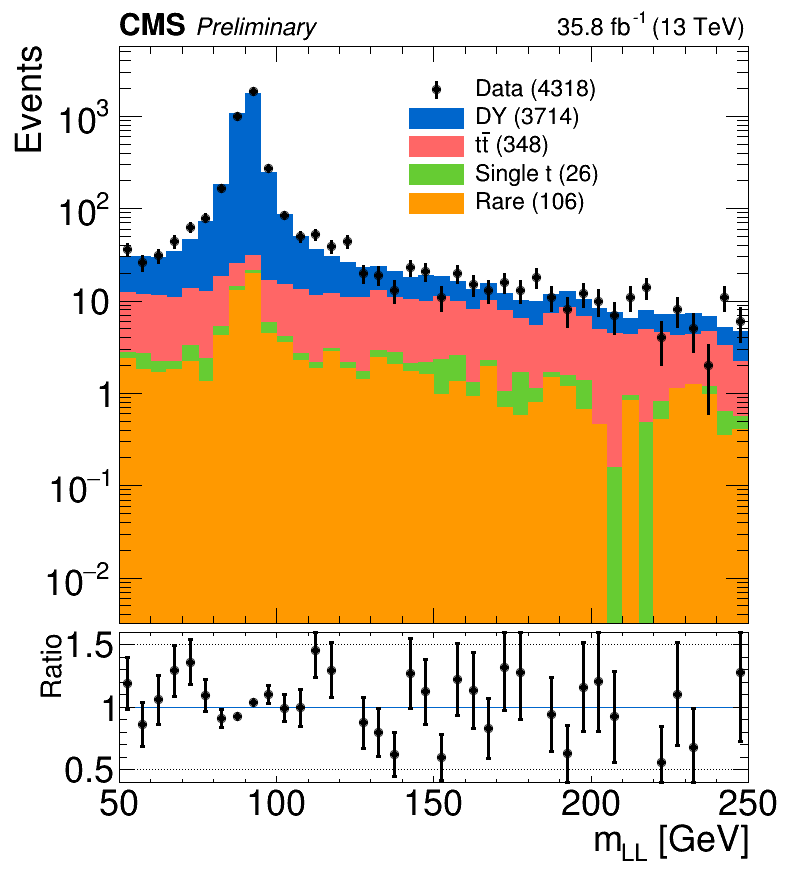
\includegraphics[width=0.40\textwidth]{znunu/fromCaleb/DataMC_Electron_LowDM_bestRecoZM_50to250_jetpt30_2016.png} \\
    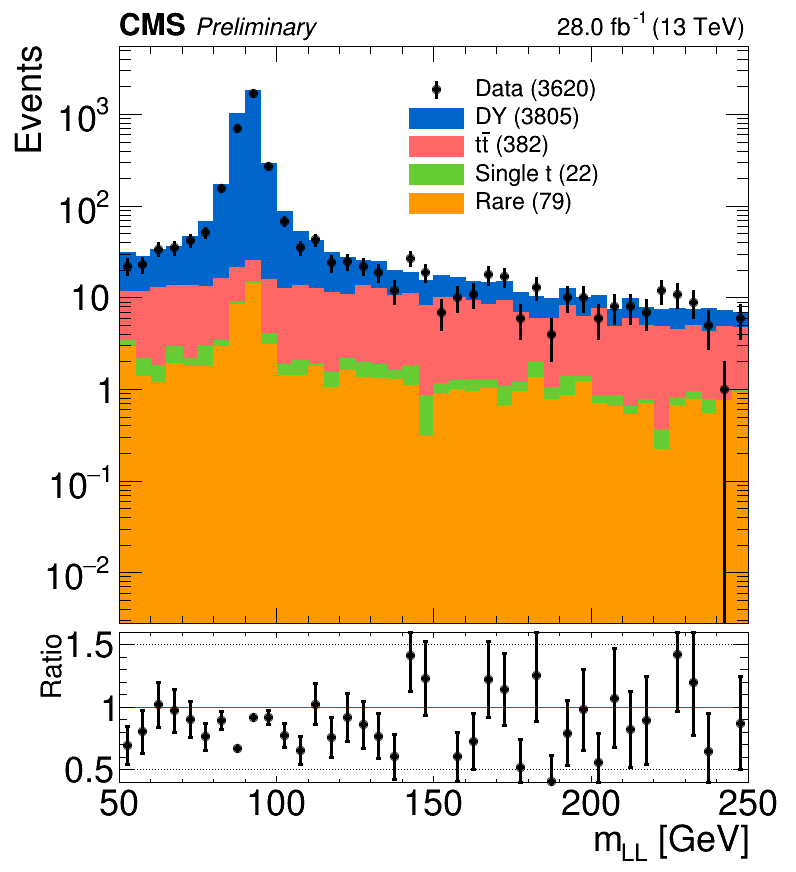
\includegraphics[width=0.40\textwidth]{znunu/fromCaleb/DataMC_Electron_LowDM_bestRecoZM_50to250_jetpt30_2017_BE.png} 
    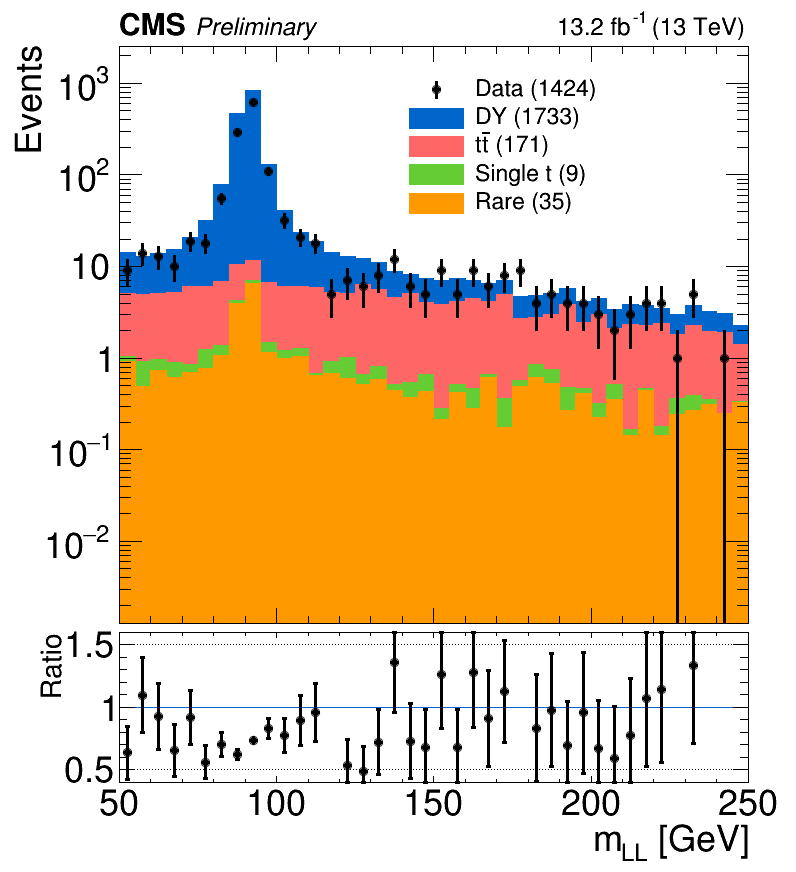
\includegraphics[width=0.40\textwidth]{znunu/fromCaleb/DataMC_Electron_LowDM_bestRecoZM_50to250_jetpt30_2017_F.png} \\
    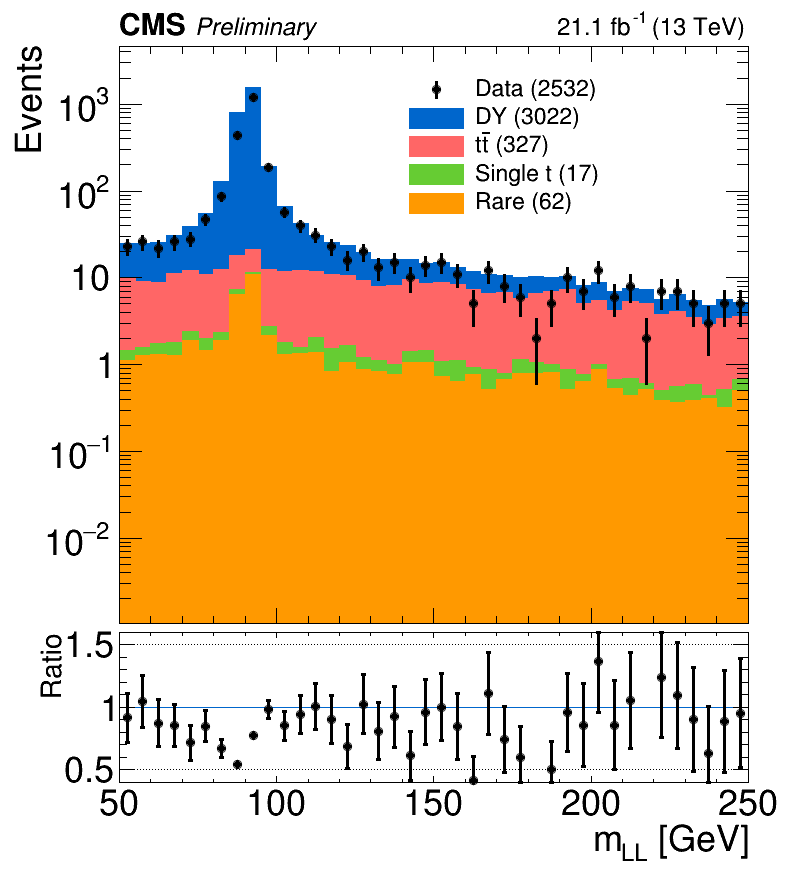
\includegraphics[width=0.40\textwidth]{znunu/fromCaleb/DataMC_Electron_LowDM_bestRecoZM_50to250_jetpt30_2018_PreHEM.png}
    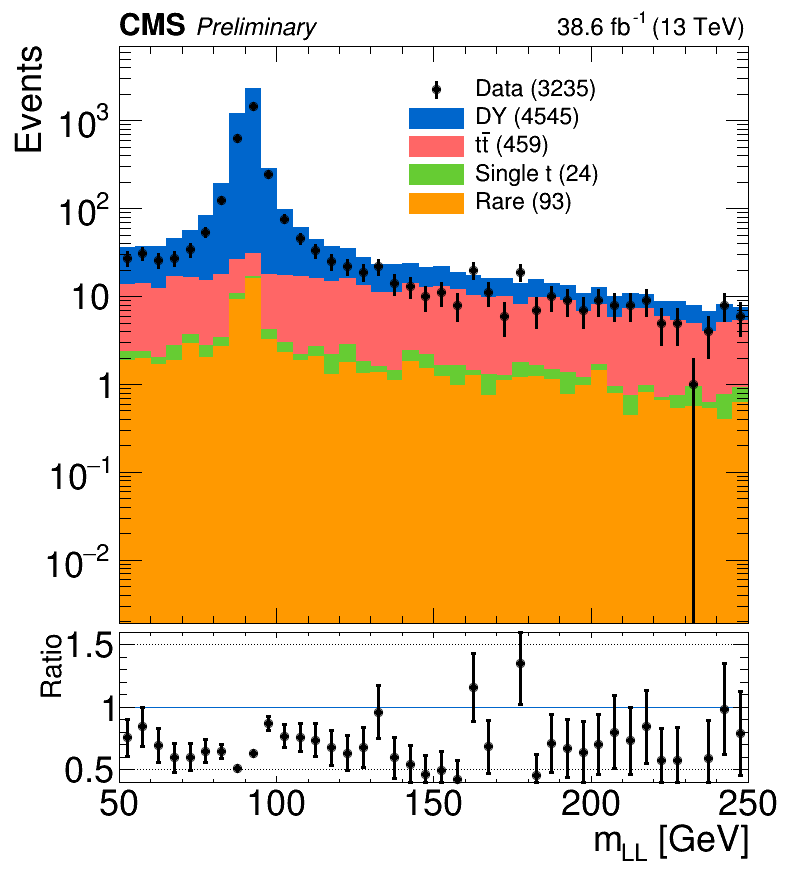
\includegraphics[width=0.40\textwidth]{znunu/fromCaleb/DataMC_Electron_LowDM_bestRecoZM_50to250_jetpt30_2018_PostHEM.png} \\
	\end{center}
	\caption[\Znunu{} Normalization in Low \dm{} for Electronss]{The \Znunu{} normalization separated by era for the electron control region. The selection is the low $\dm, \nb=0, \nsv=0$ in the electron control region.
	 }
	\label{fig:znunu-norm-lm-electron}
\end{figure}

\begin{figure}[!h]
	\begin{center}
    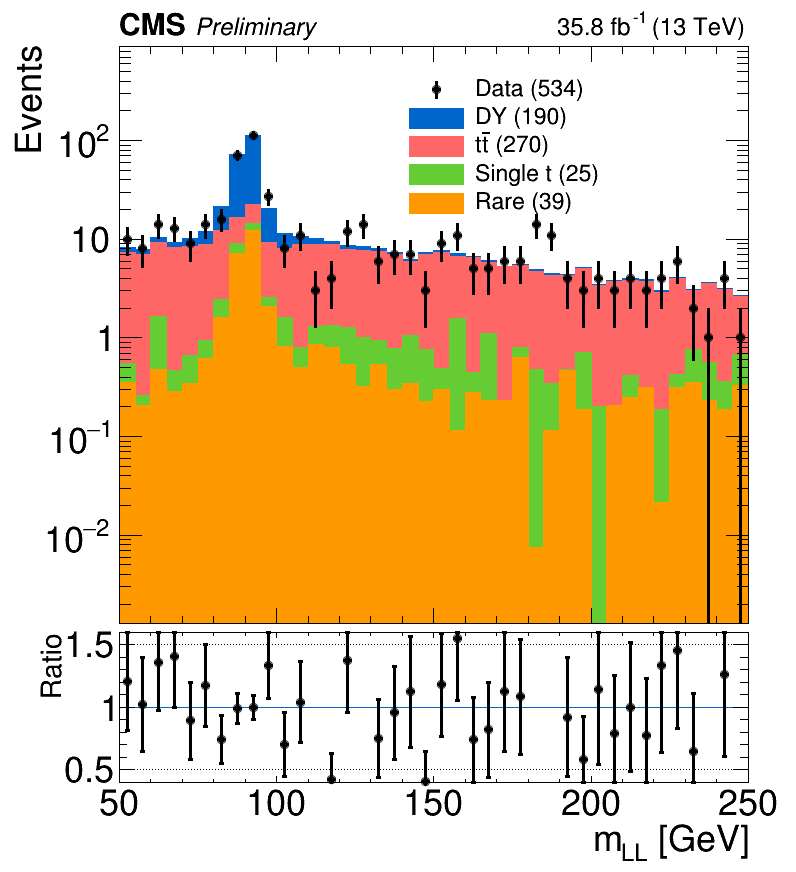
\includegraphics[width=0.40\textwidth]{znunu/fromCaleb/DataMC_Electron_HighDM_bestRecoZM_50to250_jetpt30_2016.png} \\
    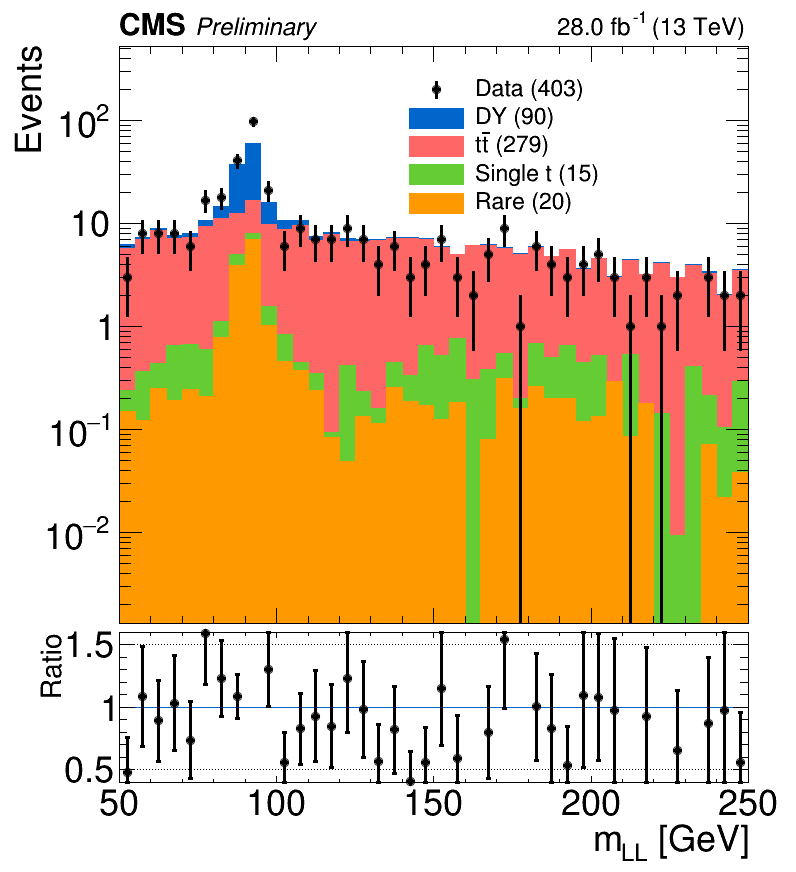
\includegraphics[width=0.40\textwidth]{znunu/fromCaleb/DataMC_Electron_HighDM_bestRecoZM_50to250_jetpt30_2017_BE.png} 
    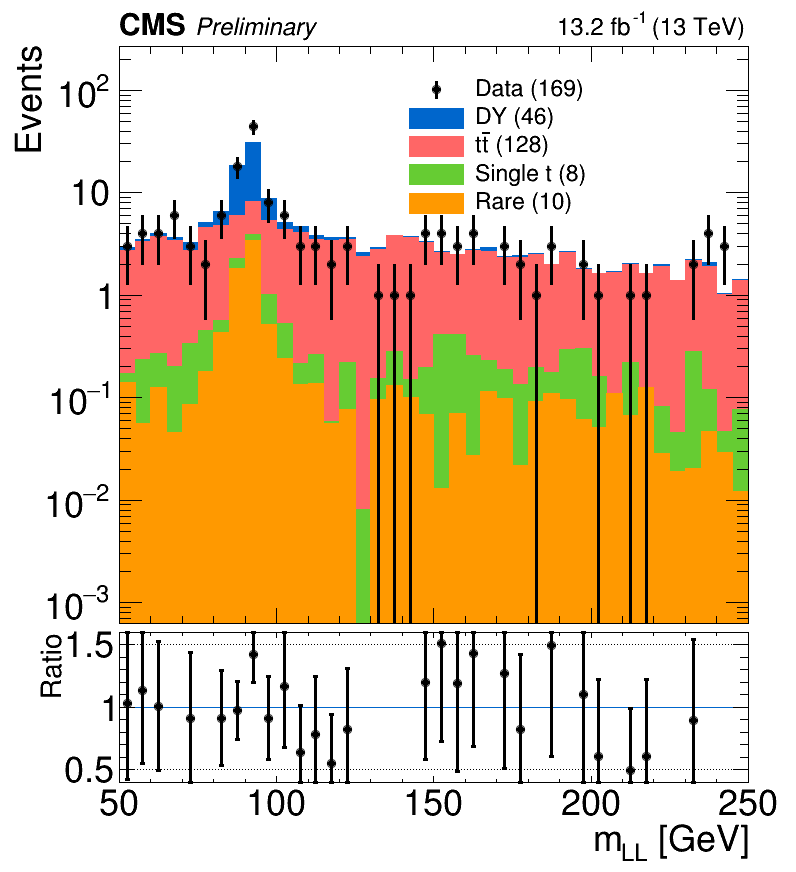
\includegraphics[width=0.40\textwidth]{znunu/fromCaleb/DataMC_Electron_HighDM_bestRecoZM_50to250_jetpt30_2017_F.png} \\
    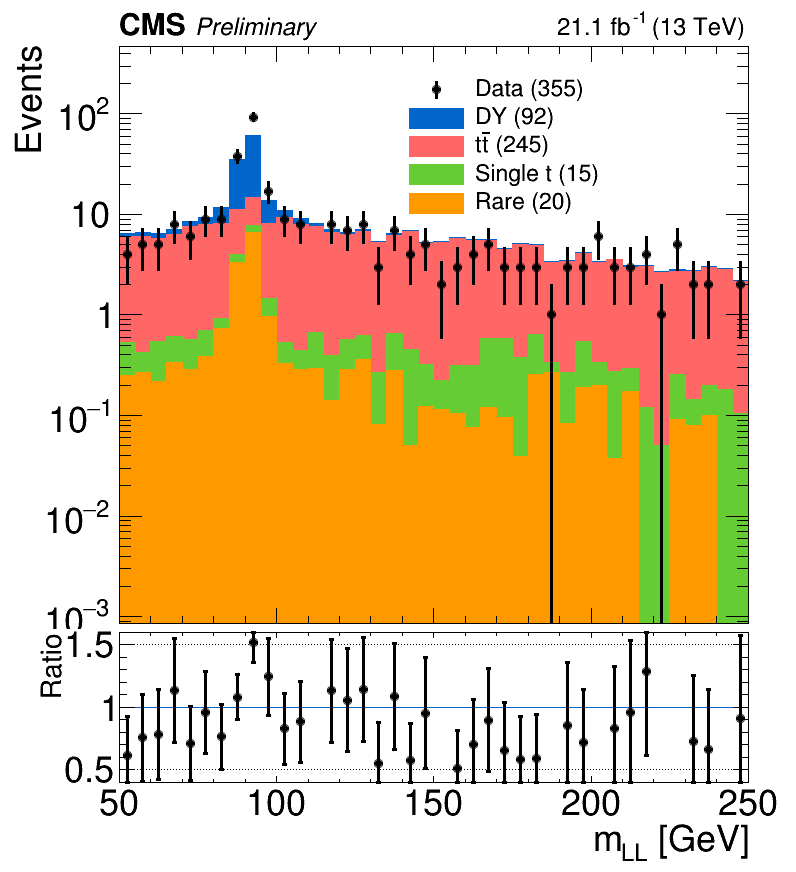
\includegraphics[width=0.40\textwidth]{znunu/fromCaleb/DataMC_Electron_HighDM_bestRecoZM_50to250_jetpt30_2018_PreHEM.png}
    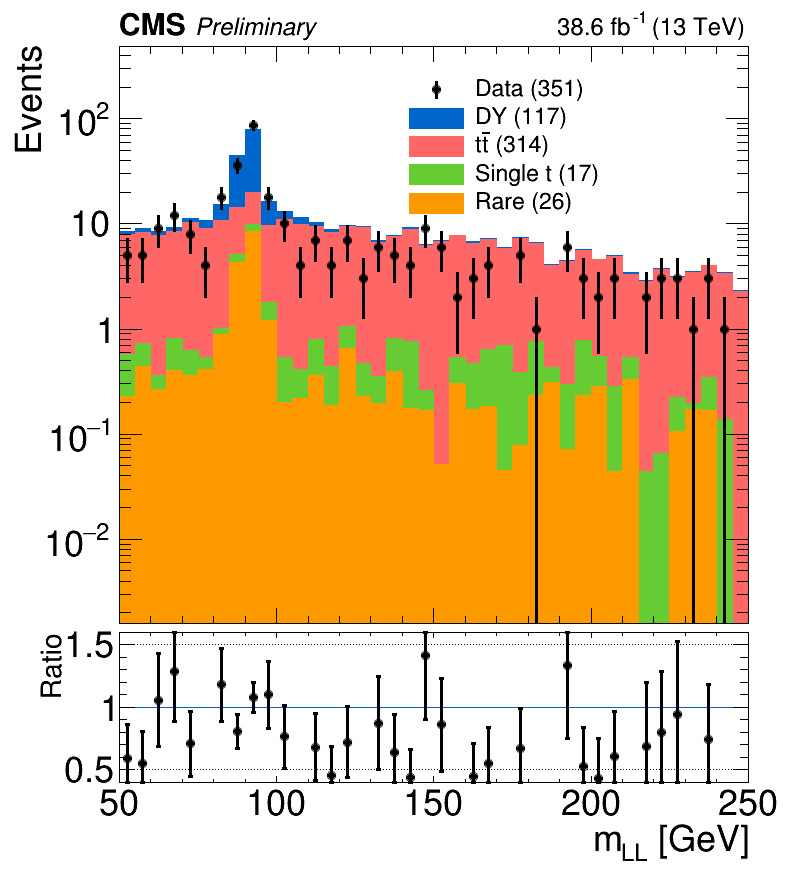
\includegraphics[width=0.40\textwidth]{znunu/fromCaleb/DataMC_Electron_HighDM_bestRecoZM_50to250_jetpt30_2018_PostHEM.png} \\
	\end{center}
	\caption[\Znunu{} Normalization in High \dm{} for Electrons]{The \Znunu{} normalization separated by era for the electron control region. The selection is the high $\dm, \nb=1, =2, \geq2,\geq3$ in the electron control region.
	 }
	\label{fig:znunu-norm-hm-electron}
\end{figure}

\begin{figure}[!h]
	\begin{center}
  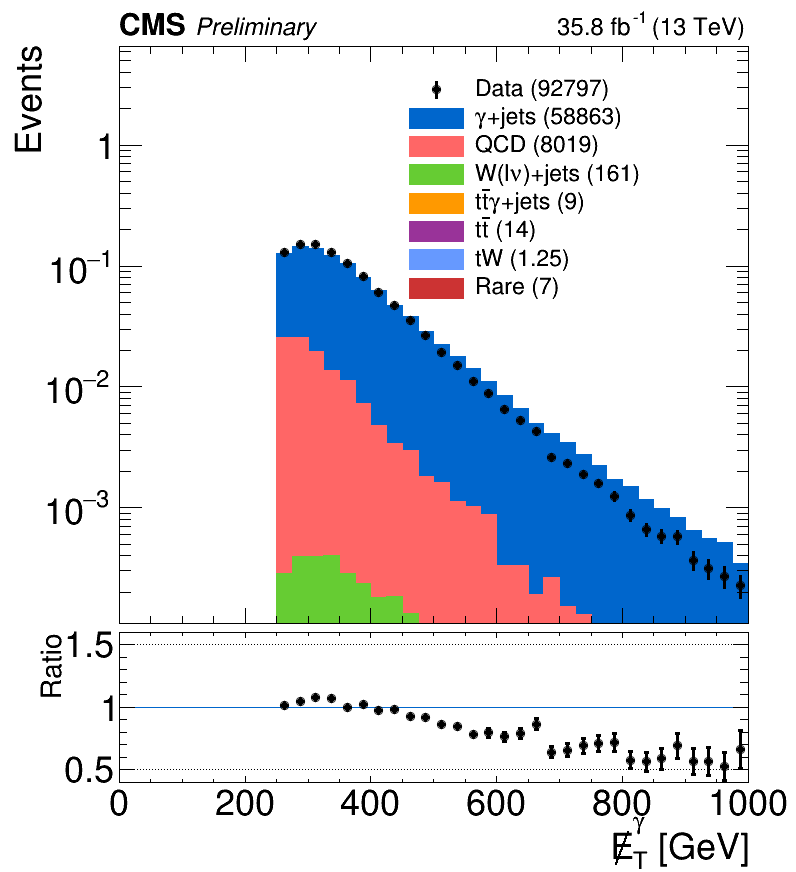
\includegraphics[width=0.40\textwidth]{znunu/fromCaleb/DataMC_Photon_LowDM_met_jetpt30_2016.png} \\
  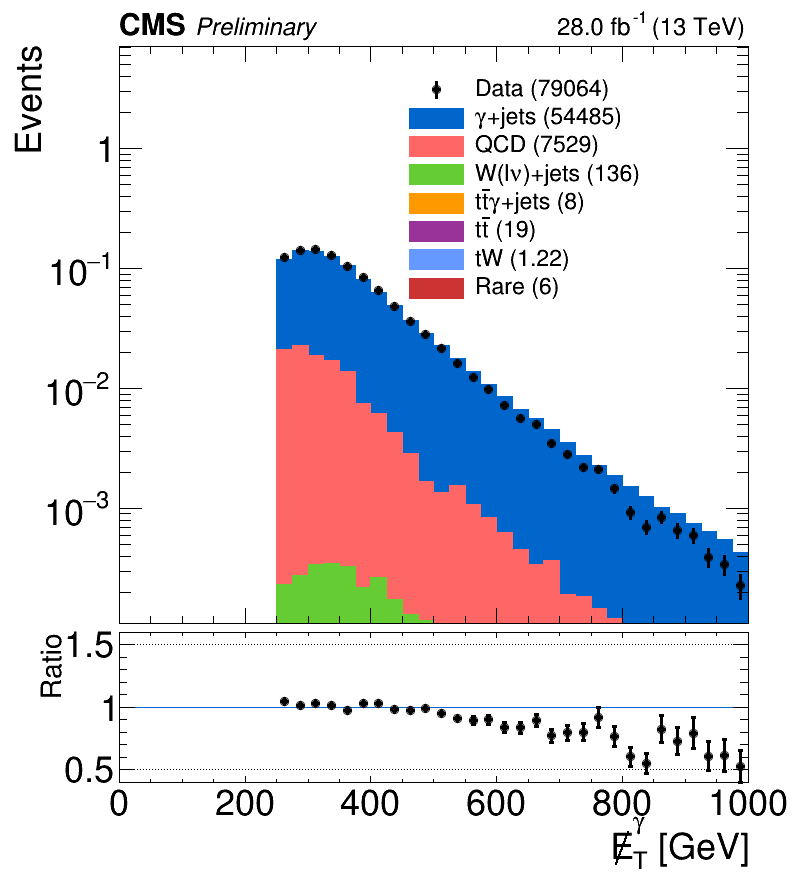
\includegraphics[width=0.40\textwidth]{znunu/fromCaleb/DataMC_Photon_LowDM_met_jetpt30_2017_BE.png} 
  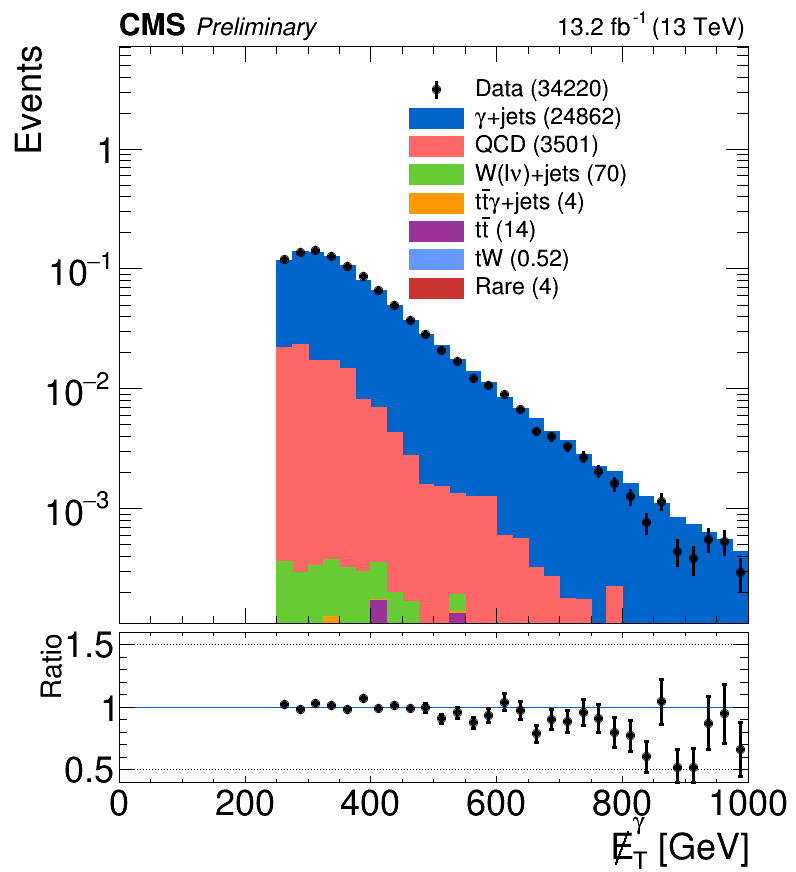
\includegraphics[width=0.40\textwidth]{znunu/fromCaleb/DataMC_Photon_LowDM_met_jetpt30_2017_F.png} \\
  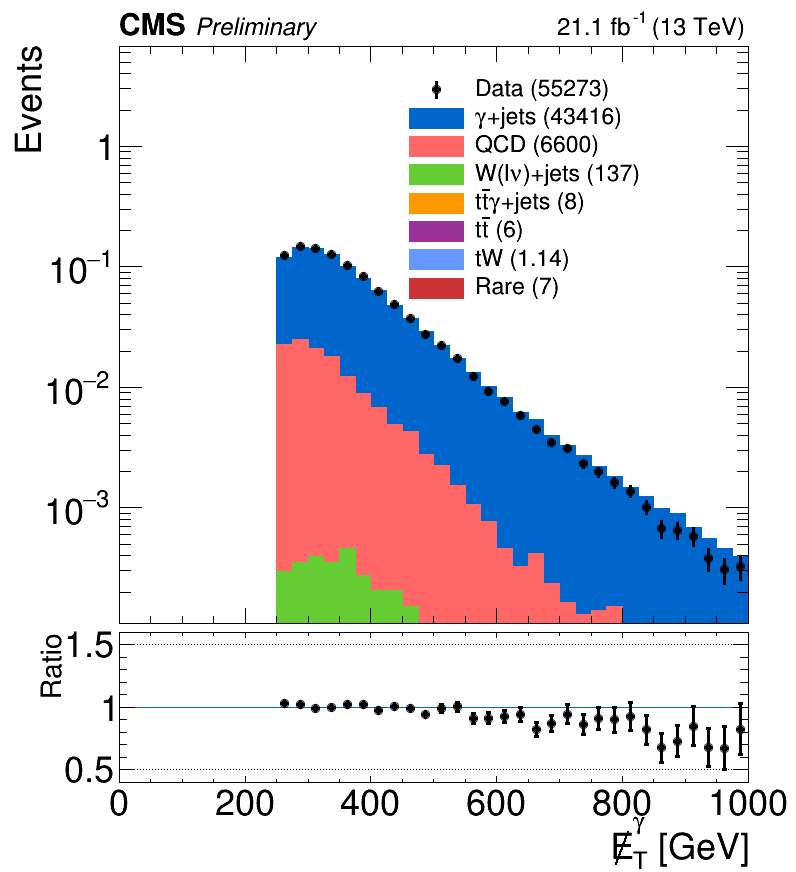
\includegraphics[width=0.40\textwidth]{znunu/fromCaleb/DataMC_Photon_LowDM_met_jetpt30_2018_PreHEM.png}
  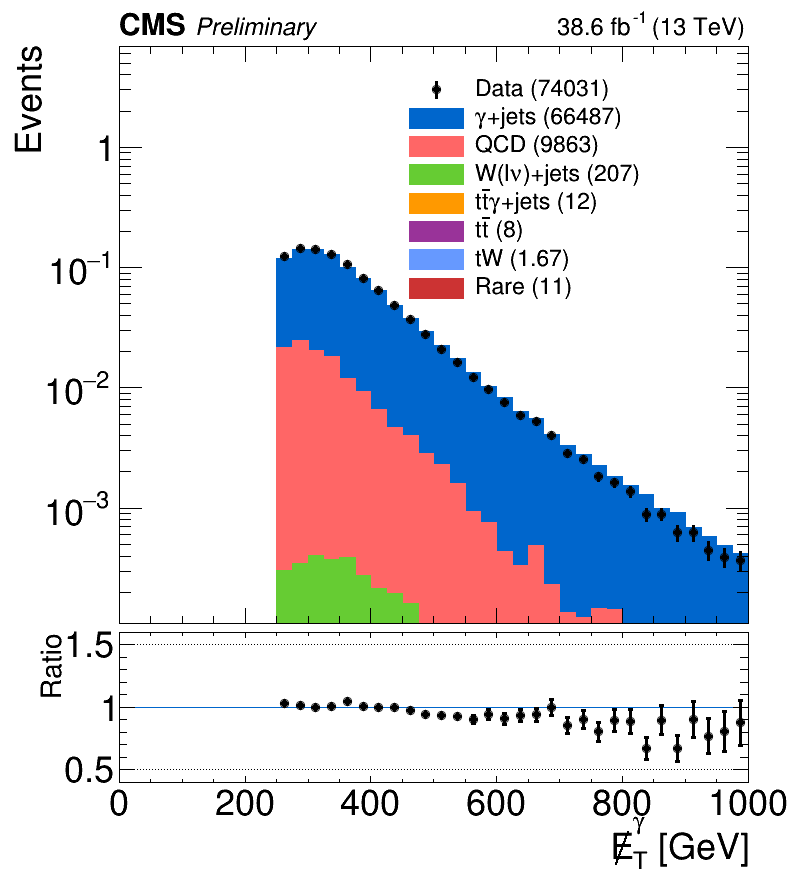
\includegraphics[width=0.40\textwidth]{znunu/fromCaleb/DataMC_Photon_LowDM_met_jetpt30_2018_PostHEM.png} \\
	\end{center}
	\caption[\Znunu{} Shape by Era]{The \Znunu{} shape corrections separated by era for the low \dm{} control region. The selection is the low $\dm, \nb=0, 2\leq\nj\leq5$ in the photon control region.
	 }
	\label{fig:znunu-shape-lm-photon}
\end{figure}

\begin{figure}[!h]
	\begin{center}
  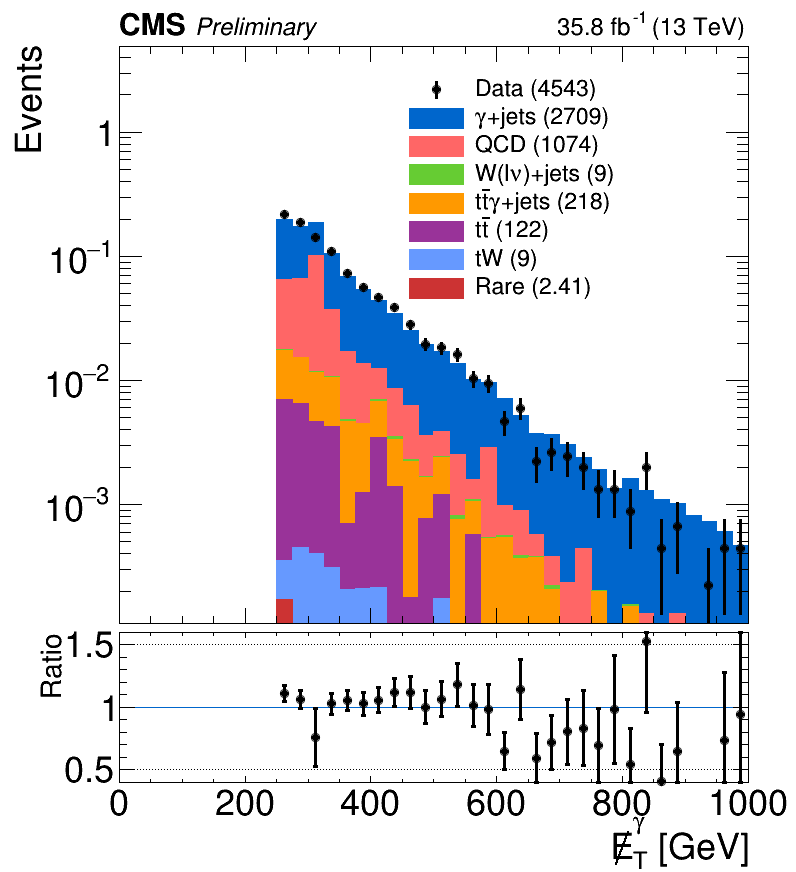
\includegraphics[width=0.40\textwidth]{znunu/fromCaleb/DataMC_Photon_HighDM_met_jetpt30_2016.png} \\
  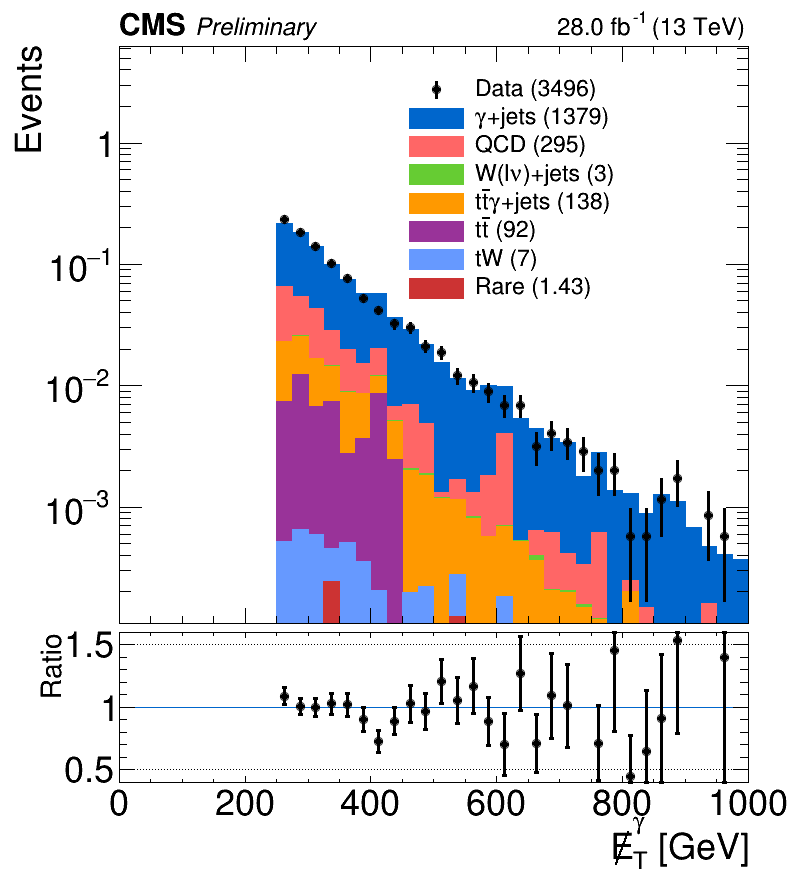
\includegraphics[width=0.40\textwidth]{znunu/fromCaleb/DataMC_Photon_HighDM_met_jetpt30_2017_BE.png} 
  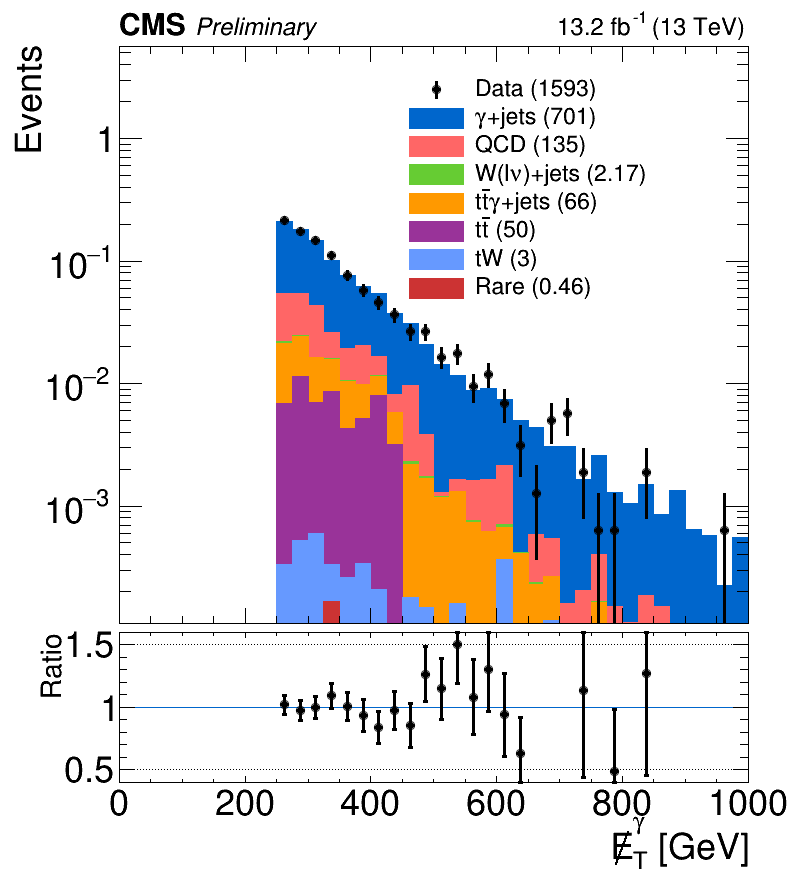
\includegraphics[width=0.40\textwidth]{znunu/fromCaleb/DataMC_Photon_HighDM_met_jetpt30_2017_F.png} \\
  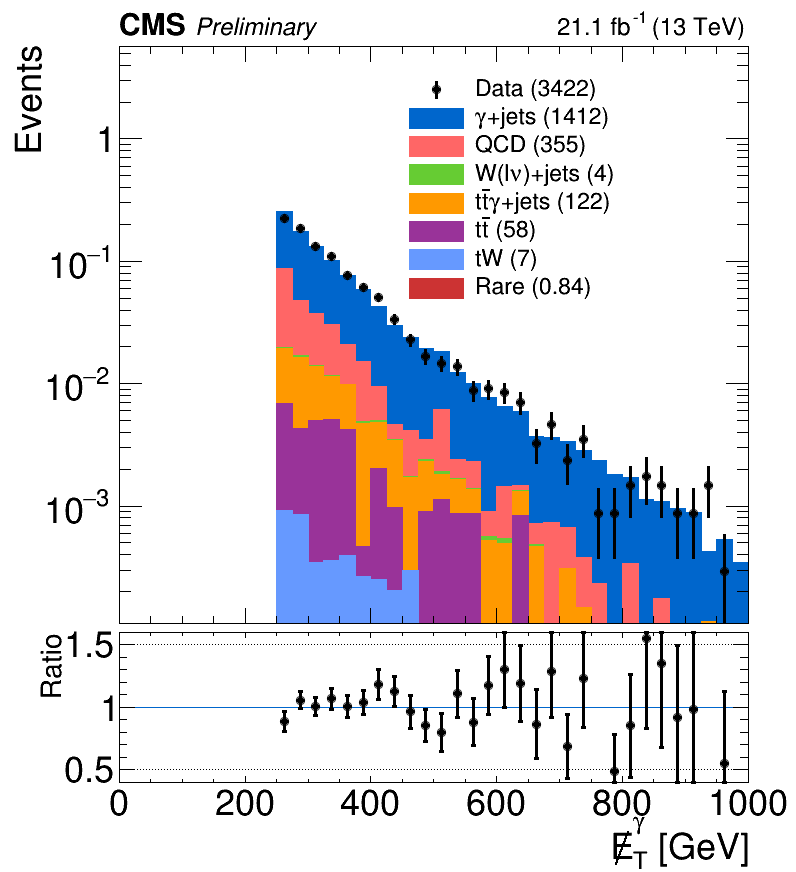
\includegraphics[width=0.40\textwidth]{znunu/fromCaleb/DataMC_Photon_HighDM_met_jetpt30_2018_PreHEM.png}
  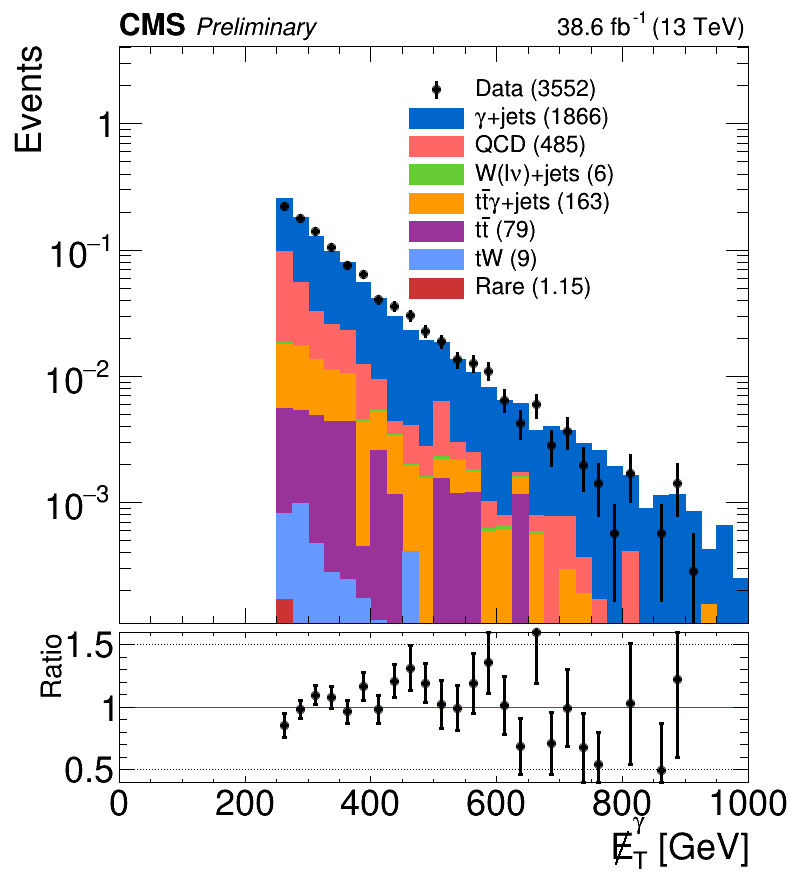
\includegraphics[width=0.40\textwidth]{znunu/fromCaleb/DataMC_Photon_HighDM_met_jetpt30_2018_PostHEM.png} \\
	\end{center}
	\caption[\Znunu{} Shape by Era]{The \Znunu{} shape corrections separated by era for the high \dm{} control region. The selection is the low $\dm, \nb=0, 2\leq\nj\leq5$ in the photon control region.
	 }
	\label{fig:znunu-shape-hm-photon}
\end{figure}
